\documentclass[12pt]{article}

% This first part of the file is called the PREAMBLE. It includes
% customizations and command definitions. The preamble is everything
% between \documentclass and \begin{document}.

\usepackage[margin=1in]{geometry}  % set the margins to 1in on all sides
\usepackage{graphicx}              % to include figures
\usepackage{amsmath}               % great math stuff
\usepackage{amsfonts}              % for blackboard bold, etc
\usepackage{amsthm}                % better theorem environments
\usepackage{amssymb} 
\usepackage{mathptmx}
\usepackage{enumerate}
\usepackage{listings}
\usepackage{xcolor}
\usepackage{forest}
\usepackage{tabularx}  

% various theorems, numbered by section

\newtheorem{thm}{Theorem}[section]
\newtheorem{lem}[thm]{Lemma}
\newtheorem{prop}[thm]{Proposition}
\newtheorem{cor}[thm]{Corollary}
\newtheorem{conj}[thm]{Conjecture}
\newtheorem{mydef}[thm]{Definition}
\lstset{
	basicstyle          =   \sffamily,          
	keywordstyle        =   \bfseries,          
	commentstyle        =   \rmfamily\itshape,  
	stringstyle         =   \ttfamily,  
	flexiblecolumns,                
	numbers             =   left,   
	showspaces          =   false,  
	numberstyle         =   \fontsize{5}{skip},    
	showstringspaces    =   false,
	captionpos          =   t,      
	frame               =   lrtb,   
}

\lstdefinestyle{cpp}{
	language        =   cpp, 
	basicstyle      =   \fontsize{5}{skip},
	numberstyle     =   \fontsize{5}{skip},
	keywordstyle    =   \color{blue},
	keywordstyle    =   [2] \color{teal},
	stringstyle     =   \color{magenta},
	commentstyle    =   \color{red}\ttfamily,
	breaklines      =   true,   
	columns         =   fixed,  
	basewidth       =   0.5em,
}
\begin{document}


\title{ CSE 102 Spring 2021\\
	Homework Assignment 6}

\author{Jaden Liu \\ 
University of California at Santa Cruz\\
Santa Cruz, CA 95064 USA }

\maketitle


\section{HW6} 
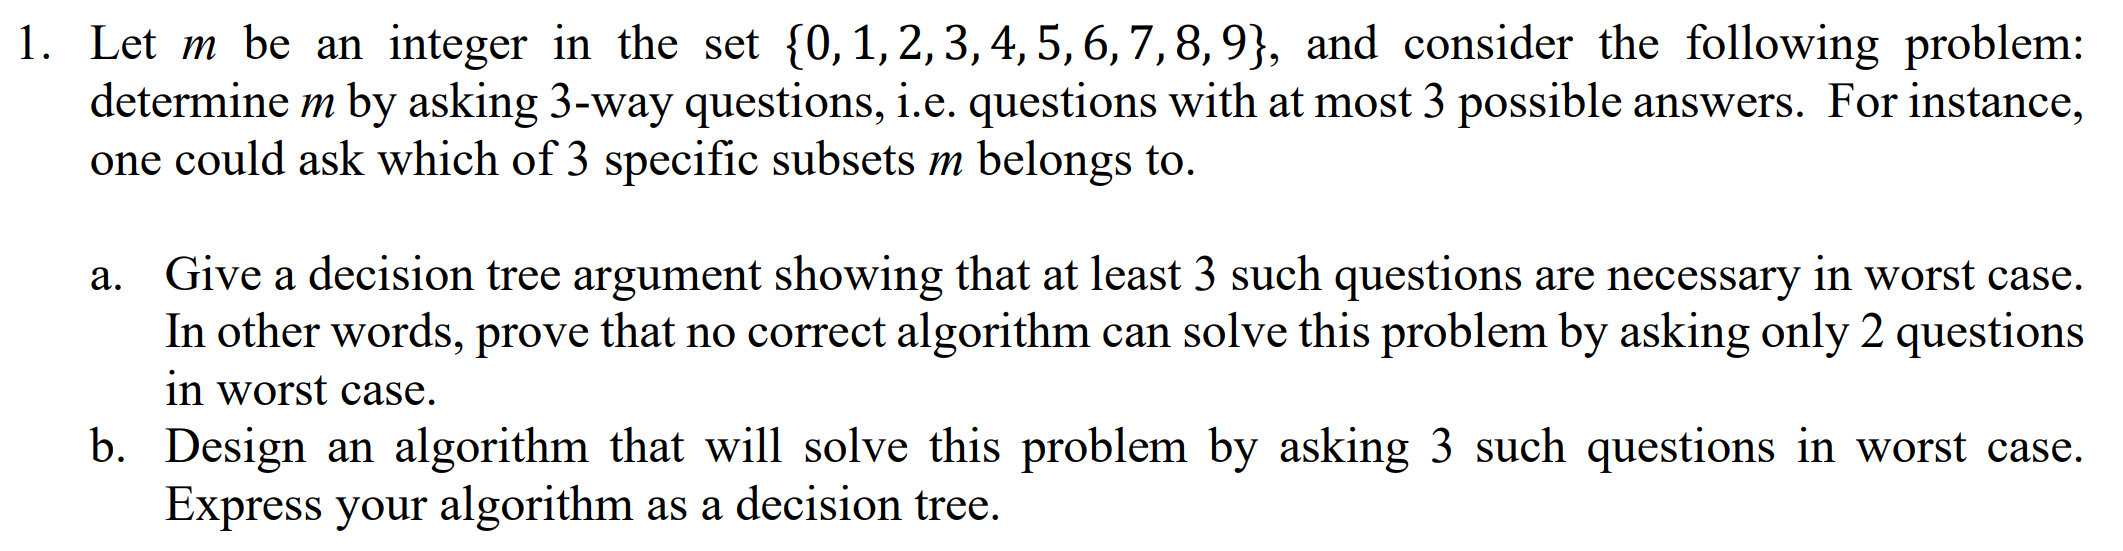
\includegraphics[scale=0.22]{1.png}
\begin{proof}[Solution for a]
	The decision tree will have $\log_{3}10$ questions at least, so we need to ask at least 3 questions. Or we can think another way: when we only ask two questions with 3 answers to each question, we have at most $3^2$ 9 answers. However, we have 10 element in the set, so we cannot get any of the element by asking less than 3 questions. 
\end{proof}
\begin{proof}[Solution for b]
	\ \\
	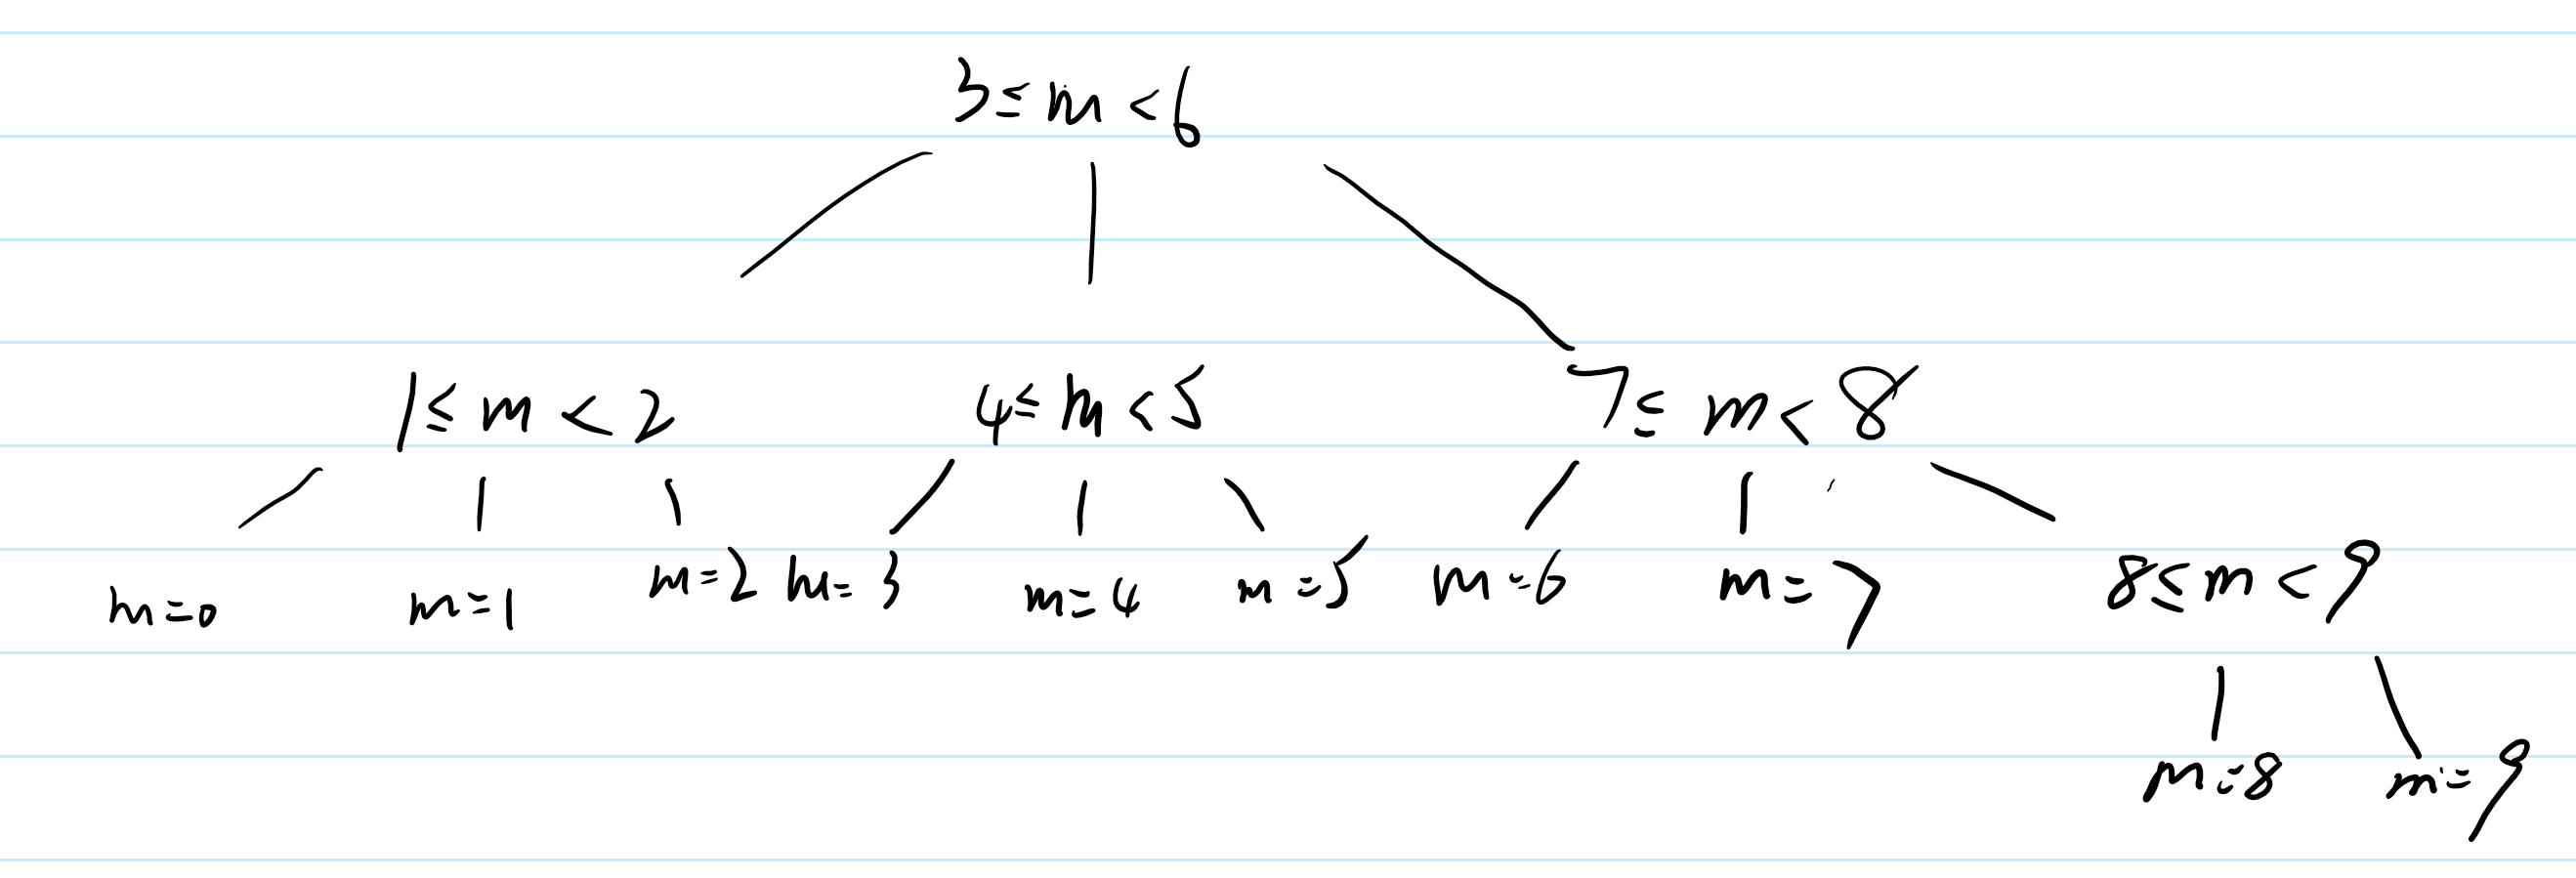
\includegraphics[scale=0.17]{1_2.png}
\end{proof}
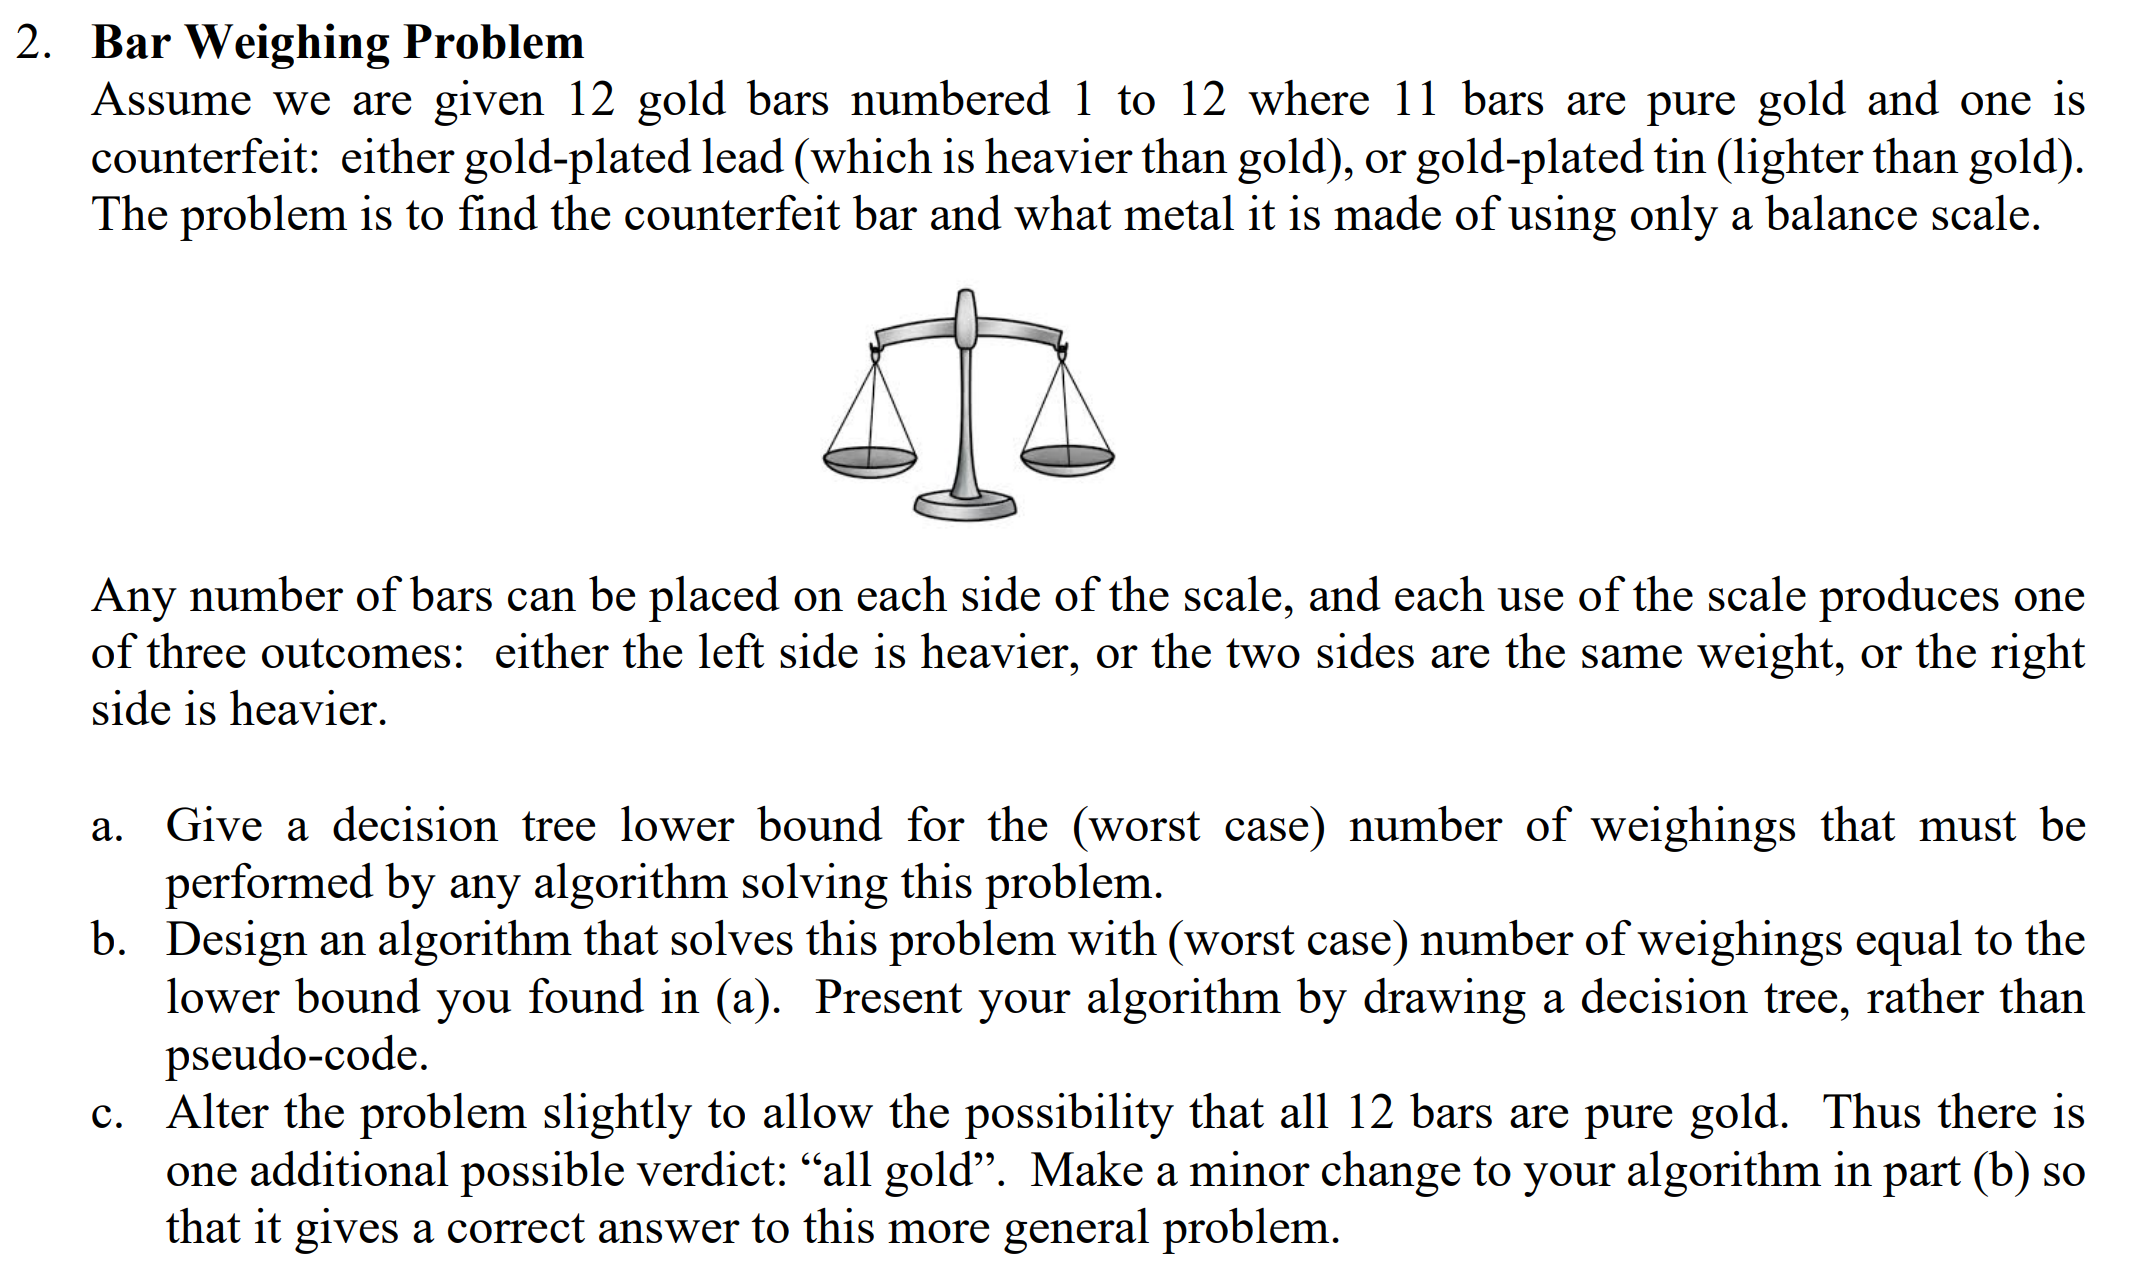
\includegraphics[scale=0.22]{2.png}
\begin{proof}[Solution for a]
	Since $\log_212\approx3.5850$, we need at least 4 weighings to solve this problem.
\end{proof}
\begin{proof}[Solution for b]
	\ \\
	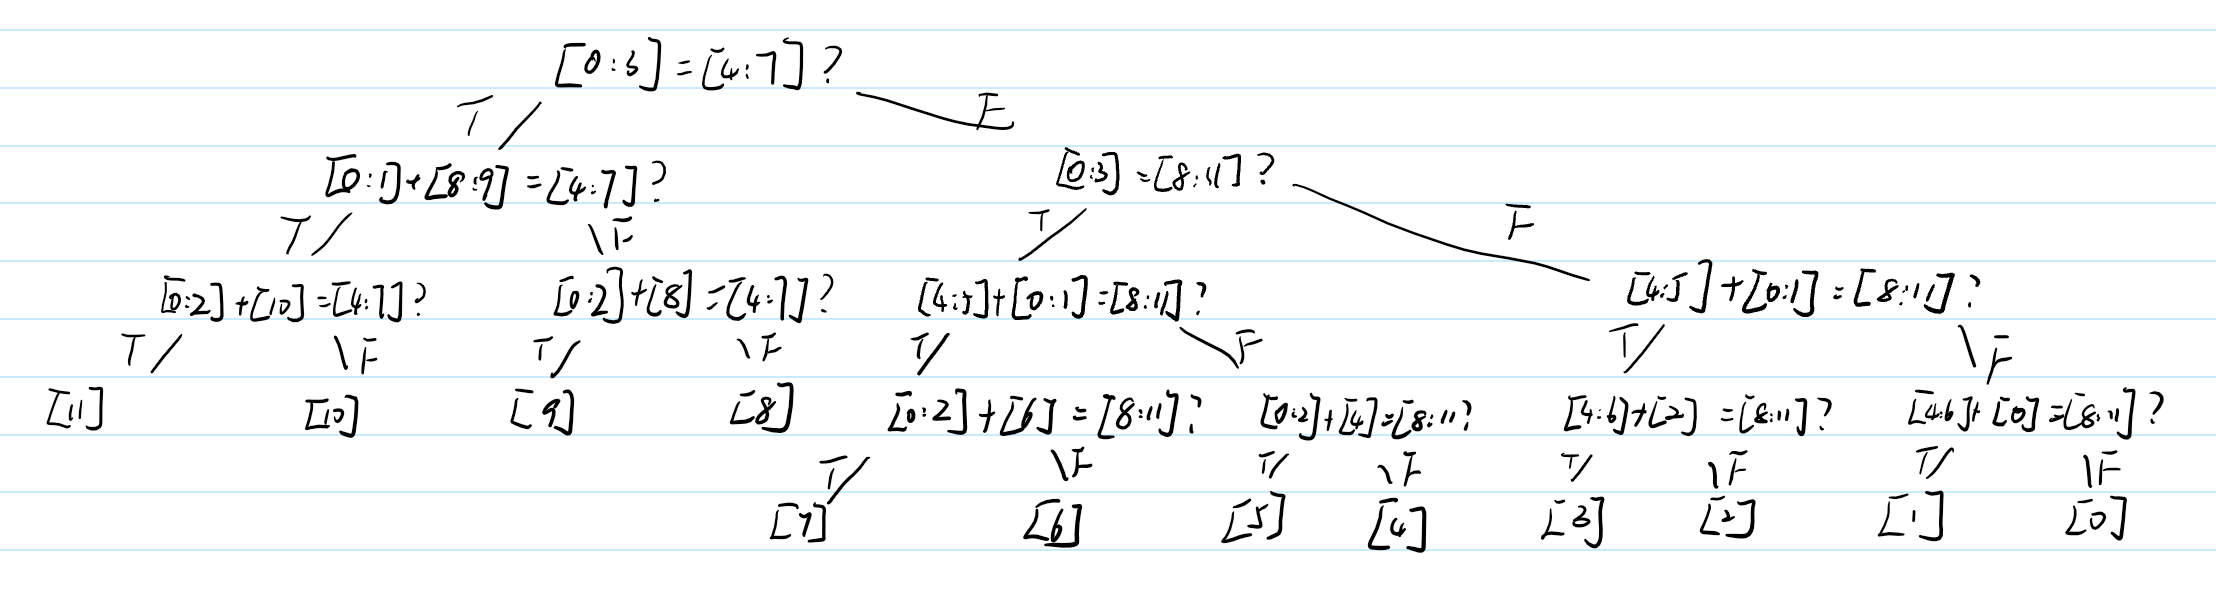
\includegraphics[scale=0.22]{2_2.png}
\end{proof}
\begin{proof}[Solution for c]
	So for our algorithm, we can add another compare process after the first step. When we compare [0:3] to [4:7] and get the result true which implicits that there is a counterfeit in [8:11]. Thus, we need to add one more process in here to determine whether [8:11] has a counterfeit, comparing either [0:3] or [4:7] with [8:11] so that we will increase our minimum comparasions to 4 times.
\end{proof}
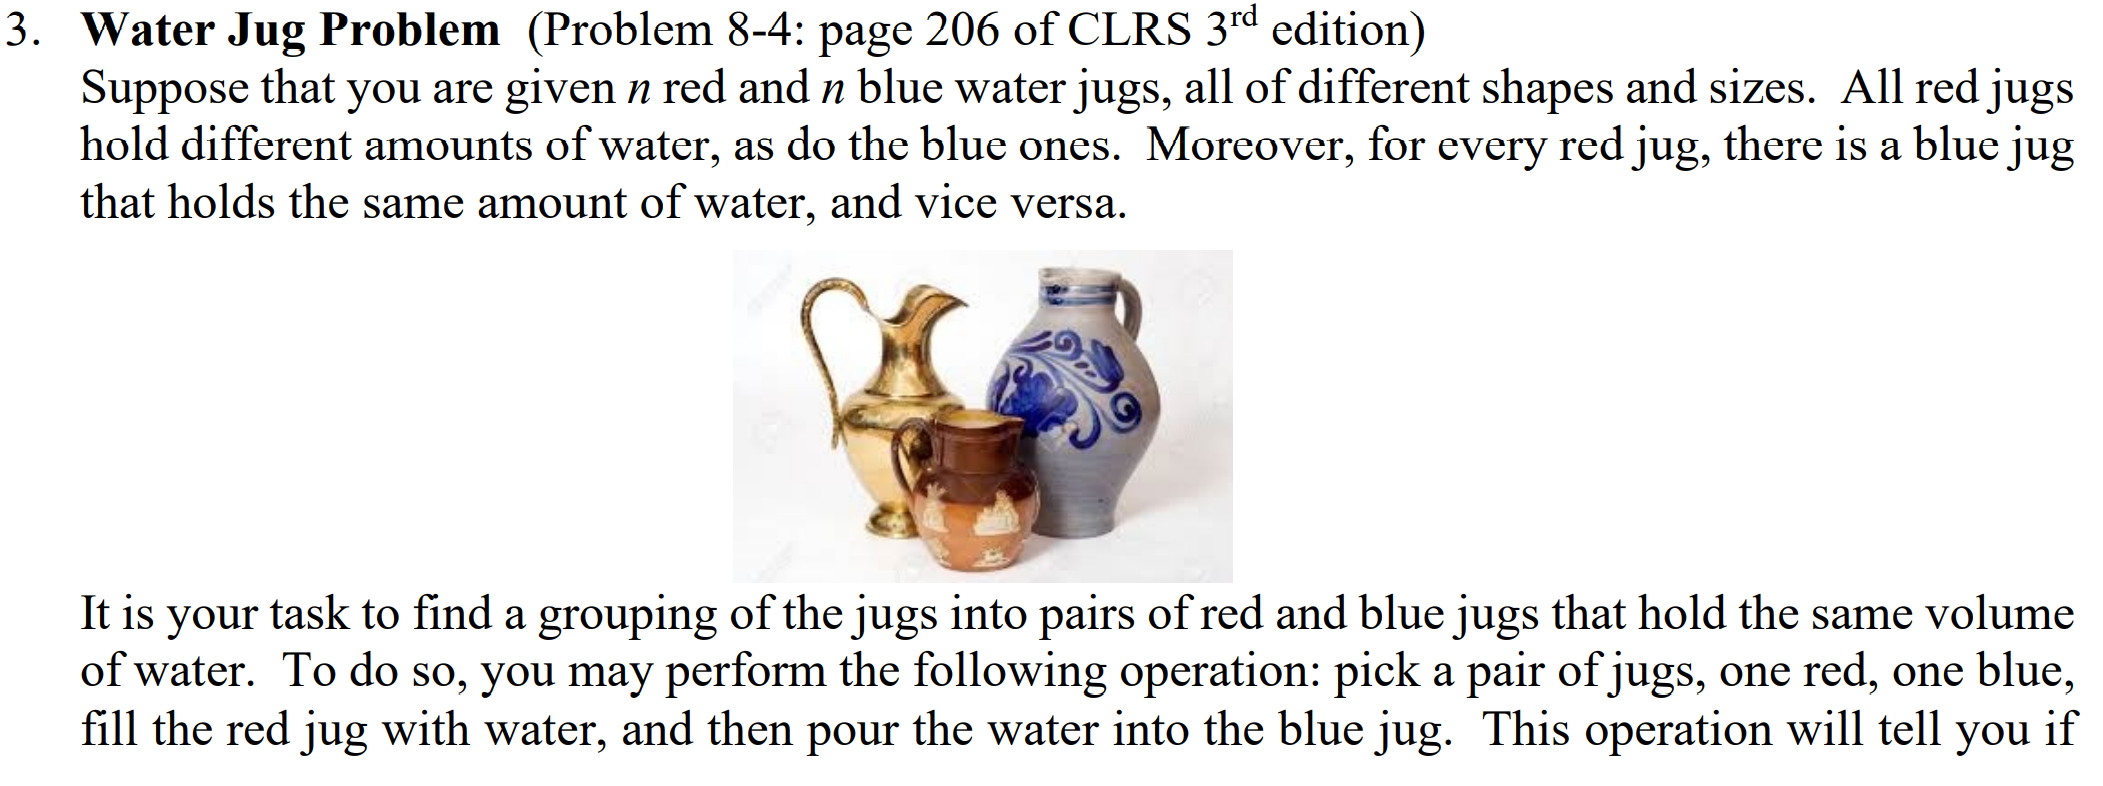
\includegraphics[scale=0.22]{3_1.png}
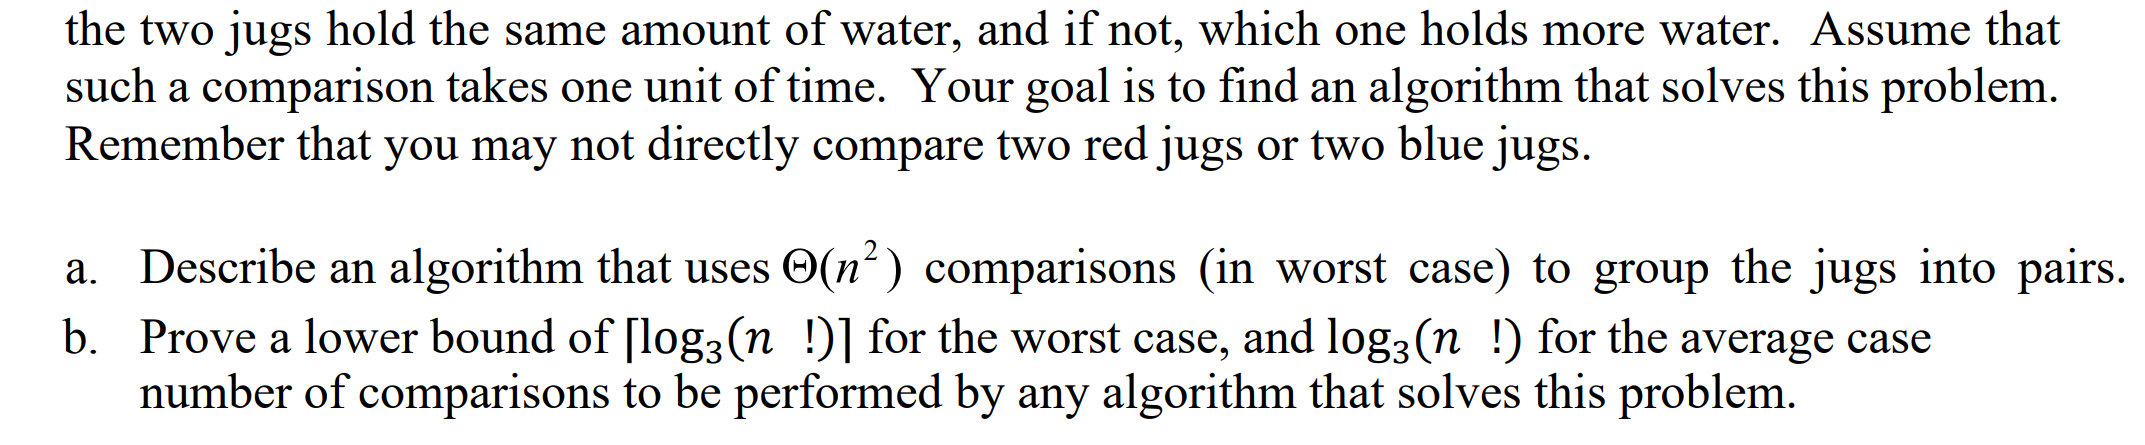
\includegraphics[scale=0.22]{3_2.png}
\begin{proof}[Solution for a]
	First we pick a red jug, then compare with one of the blue jug, stopping until we find a same capacity blue jug. Assume every time finding a pair is the in the worst case, which only make a pair in the last comparison. Thus, it takes $n+(n-1)+(n-2)+\cdots+1 = \frac{n(n+1)}{2} = \Theta(n^2)$ comparing times.
\end{proof}
\begin{proof}[Solution for b]
	We can change the problem to two array, red jugs are $R[] = [r_1,r_2,\cdots,r_n]$, while the blue jugs are $B[] = [b_1,b_2,\cdots,b_n]$. Then we just sort the two arrays, and the corresponding element in another array is the pair we need. Thus, we need $n!$ arrangement to sort this, and for each comparison, we have three result: equal, less than or greater than. Thus the worst case is $\lceil\log_{3}{n!}\rceil$. Average case needs $\log_{3}{n!}$.
\end{proof}
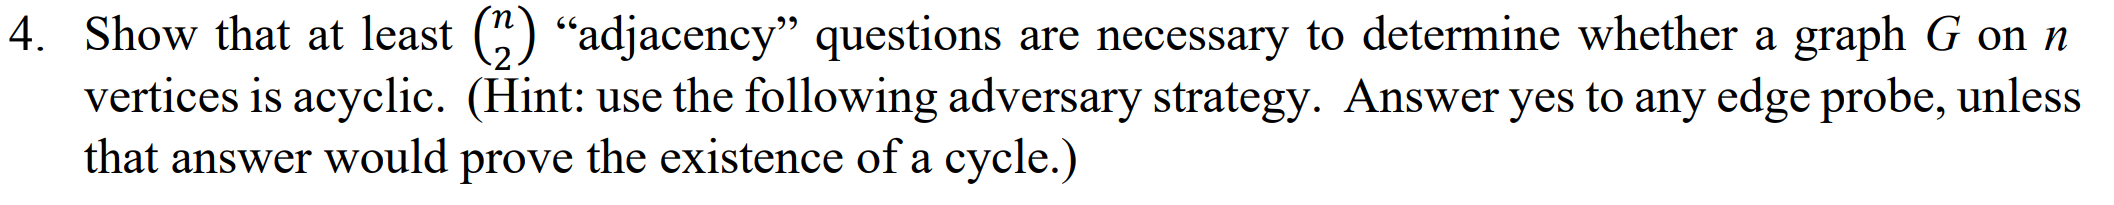
\includegraphics[scale=0.22]{4.png}
\begin{proof}[Solution]
	We can also think about the adversary strategy like the strategy of minimum spanning trees.\cite{ch} Consider the edges one at a time in increasing order of length. If adding an edge would connect the graph, declare it part of the spanning tree; otherwise, throw it away. Keep the process until we reach all ($^n_2$) edges. It's like a inverse process of Kruskal algorithm. In that case, examines all ($^n_2$) is necessary.
\end{proof}
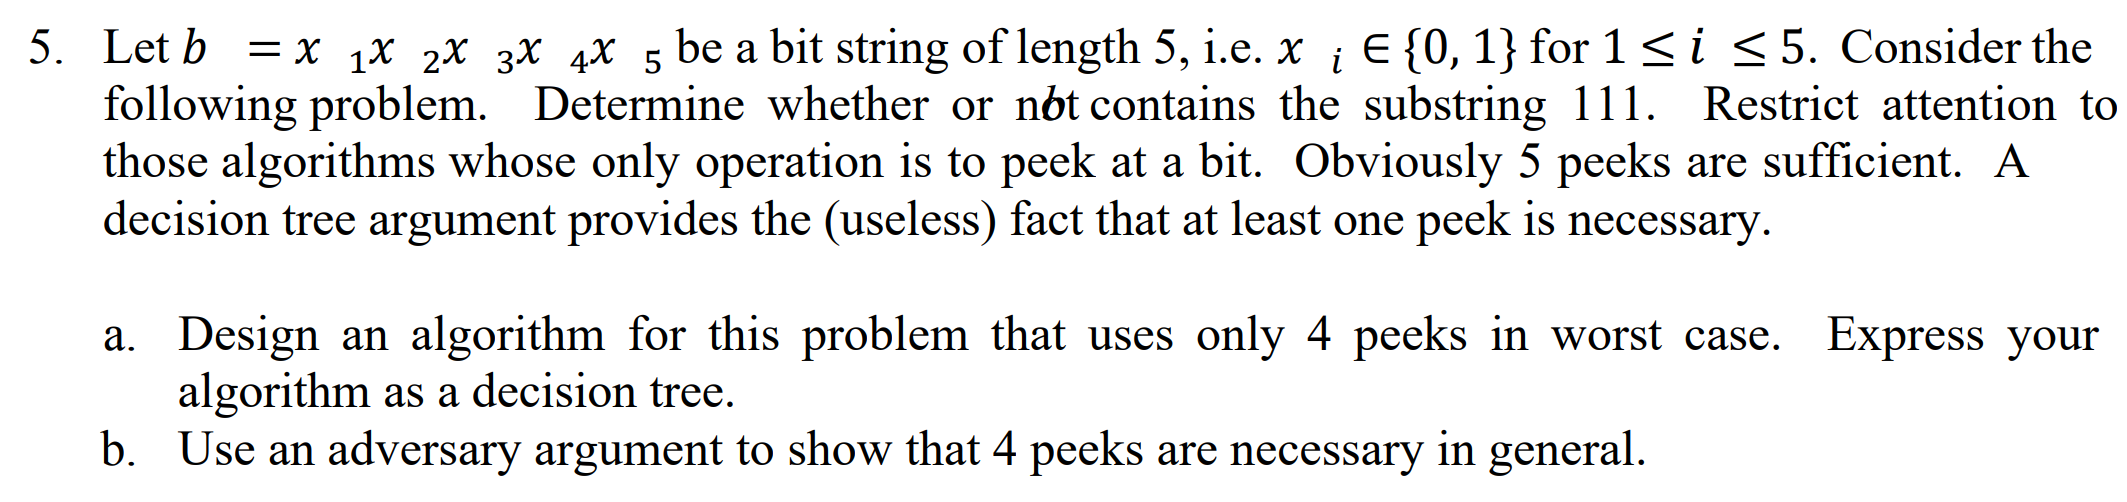
\includegraphics[scale=0.22]{5.png}
\begin{proof}[Solution for a]
	First we need to compare $x_3$ is 1, if it's not, then there cannot be a substring 111. Then compare either $x_2$ or $x_4$ then the other one.\\
	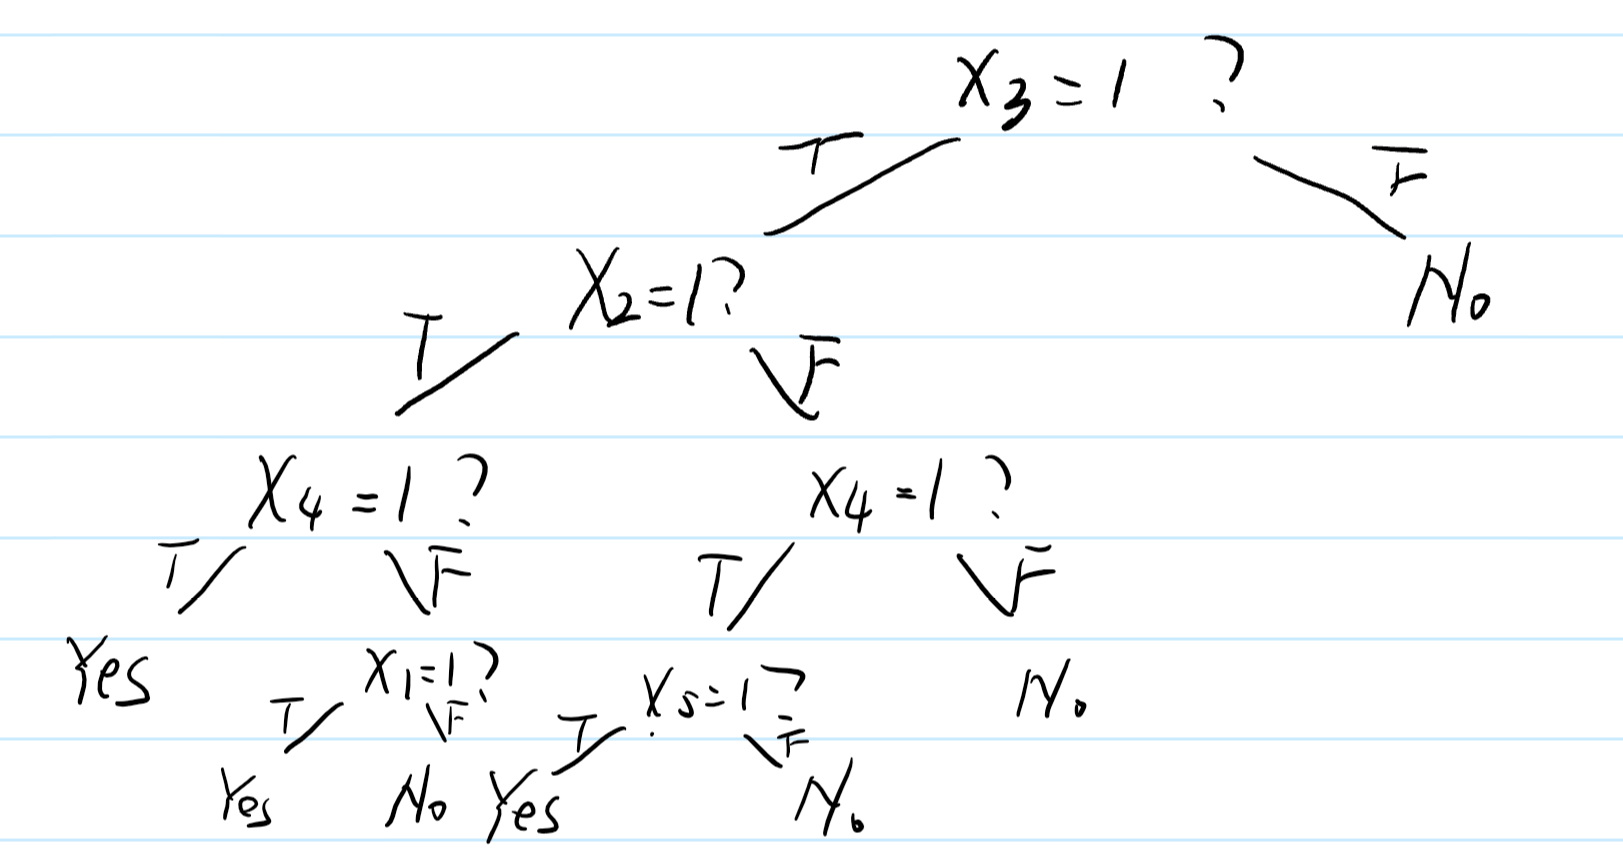
\includegraphics[scale=0.18]{5_a.png}
\end{proof}
\begin{proof}[Solution for b]
	Assume we have 00111, then we have yes, no, yes, yes; four answers in total generates there exist a substring 111.
\end{proof}
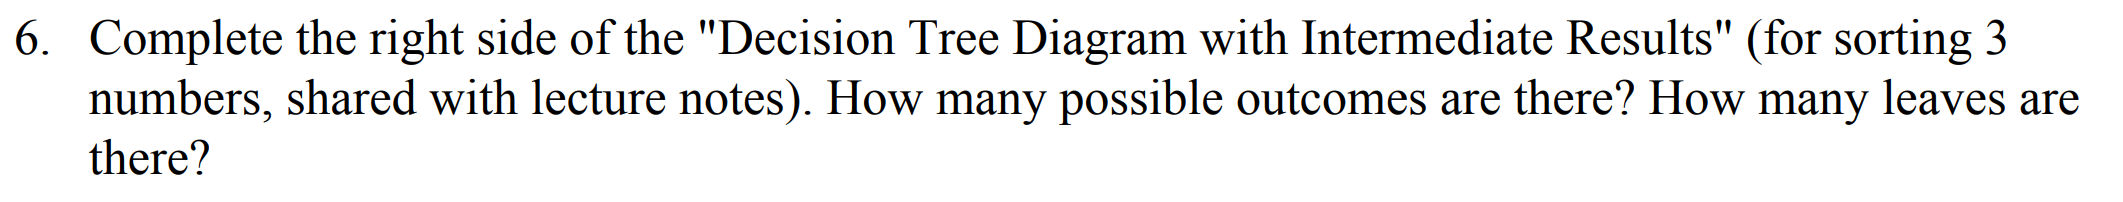
\includegraphics[scale=0.22]{6.png}
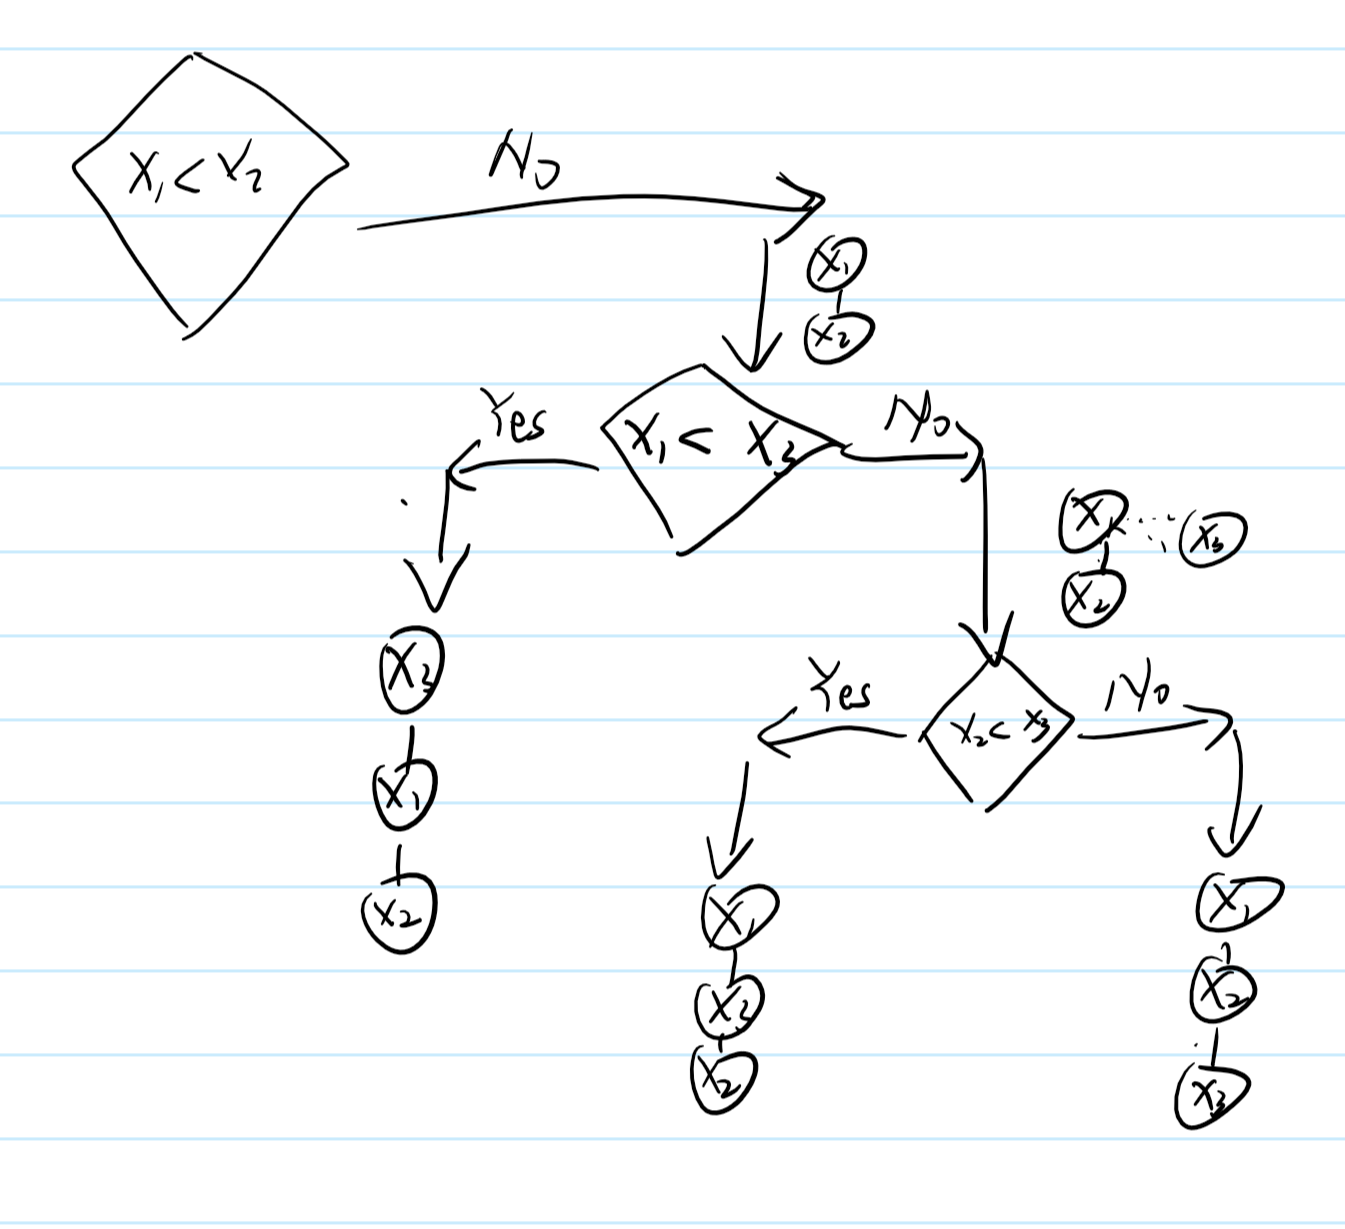
\includegraphics[scale=0.2]{6_a.png}
There are three possible outcomes and hence three leaves.
\begin{thebibliography}{ch}
	\bibitem{ch}https://courses.engr.illinois.edu/cs473/sp2010/notes/20-adversary.pdf
\end{thebibliography}


\end{document}
